\newpage
\chapter{Notions}
\label{chap:notions}

Le domaine d'activité qui entoure ce stage est très riche en termes de notions et de vocabulaire. Afin de mieux comprendre de quoi il va être question tout au long de ce rapport, il est nécessaire d'en définir les notions de base.

\paragraph{Réalité virtuelle}
La réalité virtuelle plus communément appelé \emph{Virtual Reality (VR)} désigne l'ensemble des environnements purement numériques (fig~\ref{fig:realityspectrum}), qu'ils soient réalistes ou non, dans lesquels aucune interaction avec l'environnement réel n'est possible et inversement. Cette réalité se base très généralement sur un casque \emph{Head Mounted Display (HMD)} dont l'utilisateur doit se munir afin d'être immergé dans un monde numérique avec lequel il peut interagir. Dans la réalité virtuelle, l'immersion est une notion importe lorsqu'il s'agit de la différenciée d'un simple programme informatique.

\begin{figure}[H]
\centering
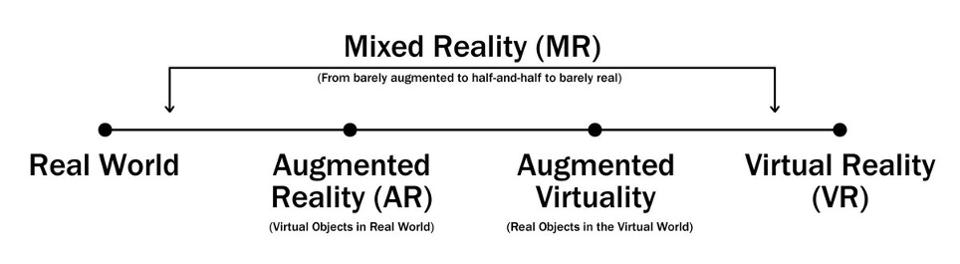
\includegraphics[width=\linewidth]{images/RealitySpectrum}
\caption{Représentation de continuum de la virtualité par Milgram et Kishino, 1995\cite{milgram1995augmented}}
\label{fig:realityspectrum}
\end{figure}

\paragraph{Réalité augmentée}
La réalité augmentée plus communément appelé \emph{Augmented Reality (AR)} quant a elle est un sous domaine de la réalité virtuelle. L'idée de la réalité augmentée est de venir superposer à l'environnement réel des éléments virtuels. Ces éléments vont alors venir "augmenter" notre monde en apportant le plus souvent des compléments d'informations. Elle est donc qualifié de sous domaine de la réalité virtuelle car l'utilisateur n'est plus immergé dans un environnement complètement numérique mais du contenu virtuel est ajouté en contexte à la vision réelle. Par abus de langage le terme de réalité augmentée est souvent utilisé pour parler de réalité mixte dont la notion est détaillé dans cette partie.
Il faut noter que ce type de réalité ne se base pas uniquement sur des \emph{HMD} mais peut être aussi apprécié à l'aide d'un téléphone par exemple (fig~\ref{fig:AR}).

\begin{figure}[H]
\centering
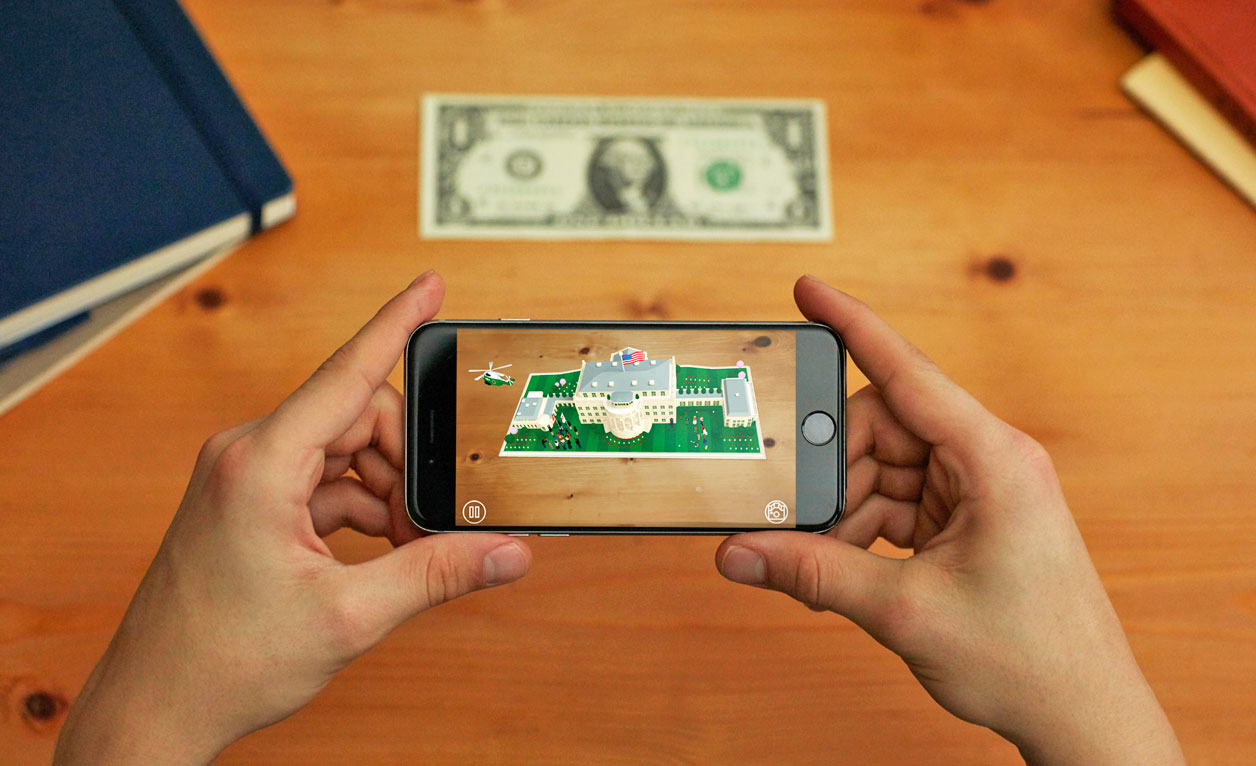
\includegraphics[width=0.55\textwidth]{images/AR}
\caption{Réalité augmentée vu au travers d'un téléphone\protect\footnotemark}\label{fig:AR}
\end{figure}
\footnotetext{Source: \href{https://www.engadget.com}{https://www.engadget.com}}

\paragraph{Réalité mixte}
La réalité mixte, ou hybride, plus communément appelé \emph{Mixed Reality (MR)}, ou \emph{Crossed Reality (XR)}, est la fusion parfaite de l'environnement numérique et de l'environnement physique (fig~\ref{fig:realityspectrum}). Dans ce "nouvel" environnement, les objets physiques et numériques coexistent et peuvent interagir entre eux et par exemple une table peut devenir une plateforme pour un personnage virtuel (fig~\ref{fig:youngconker}). Souvent confondu avec la réalité augmentée, cette dernière se différencie car elle ne propose pas seulement une visualisation des objets numériques, elle propose aussi des méthodes d'interactions avec ce contenu et c'est cette notion d'interaction qui permet de la différencier. A l'heure actuelle la réalité mixte nécessite un dispositif de type \emph{HMD} pour être appréciée comme par exemple  l'\texttt{HoloLens} de \texttt{Microsoft}.

\begin{figure}[H]
\centering
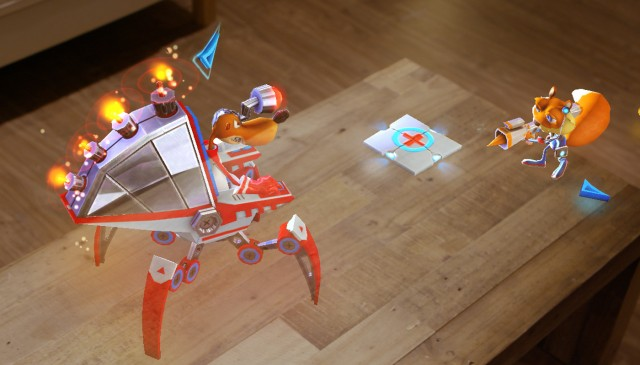
\includegraphics[scale=0.4]{images/youngconker}
\caption{Asobo Studio\texttrademark - Young Conker\copyright}
\label{fig:youngconker}
\end{figure}

\paragraph{Réalité augmentée vue au travers}
% Trouver qui l'a inventé et quand
La réalité augmentée vue au travers, plus communément appelé \emph{See Through Augmented Reality (STAR)} est une technique de visualisation de la réalité augmentée ou les éléments numériques sont vu au travers d'un écran (fig~\ref{sub:STARGO}) ou d'un \emph{HMD} (fig~\ref{sub:STARHolo}). C'est le type de visualisation le plus  utilisé actuellement. L'un des défauts majeur de ce type de visualisation est que la plus part du temps, chaque utilisateur a besoin de son propre écran ou casque pour pouvoir en profiter pleinement ce qui limite grandement les expériences collaboratives. Aussi les principaux défauts liés aux écrans s'appliquent aussi, a savoir fatigue visuel etc.  

\begin{figure}[H]
    \centering
	\subfloat[Pokémon GO - Vue au travers téléphone\protect\footnotemark]{
      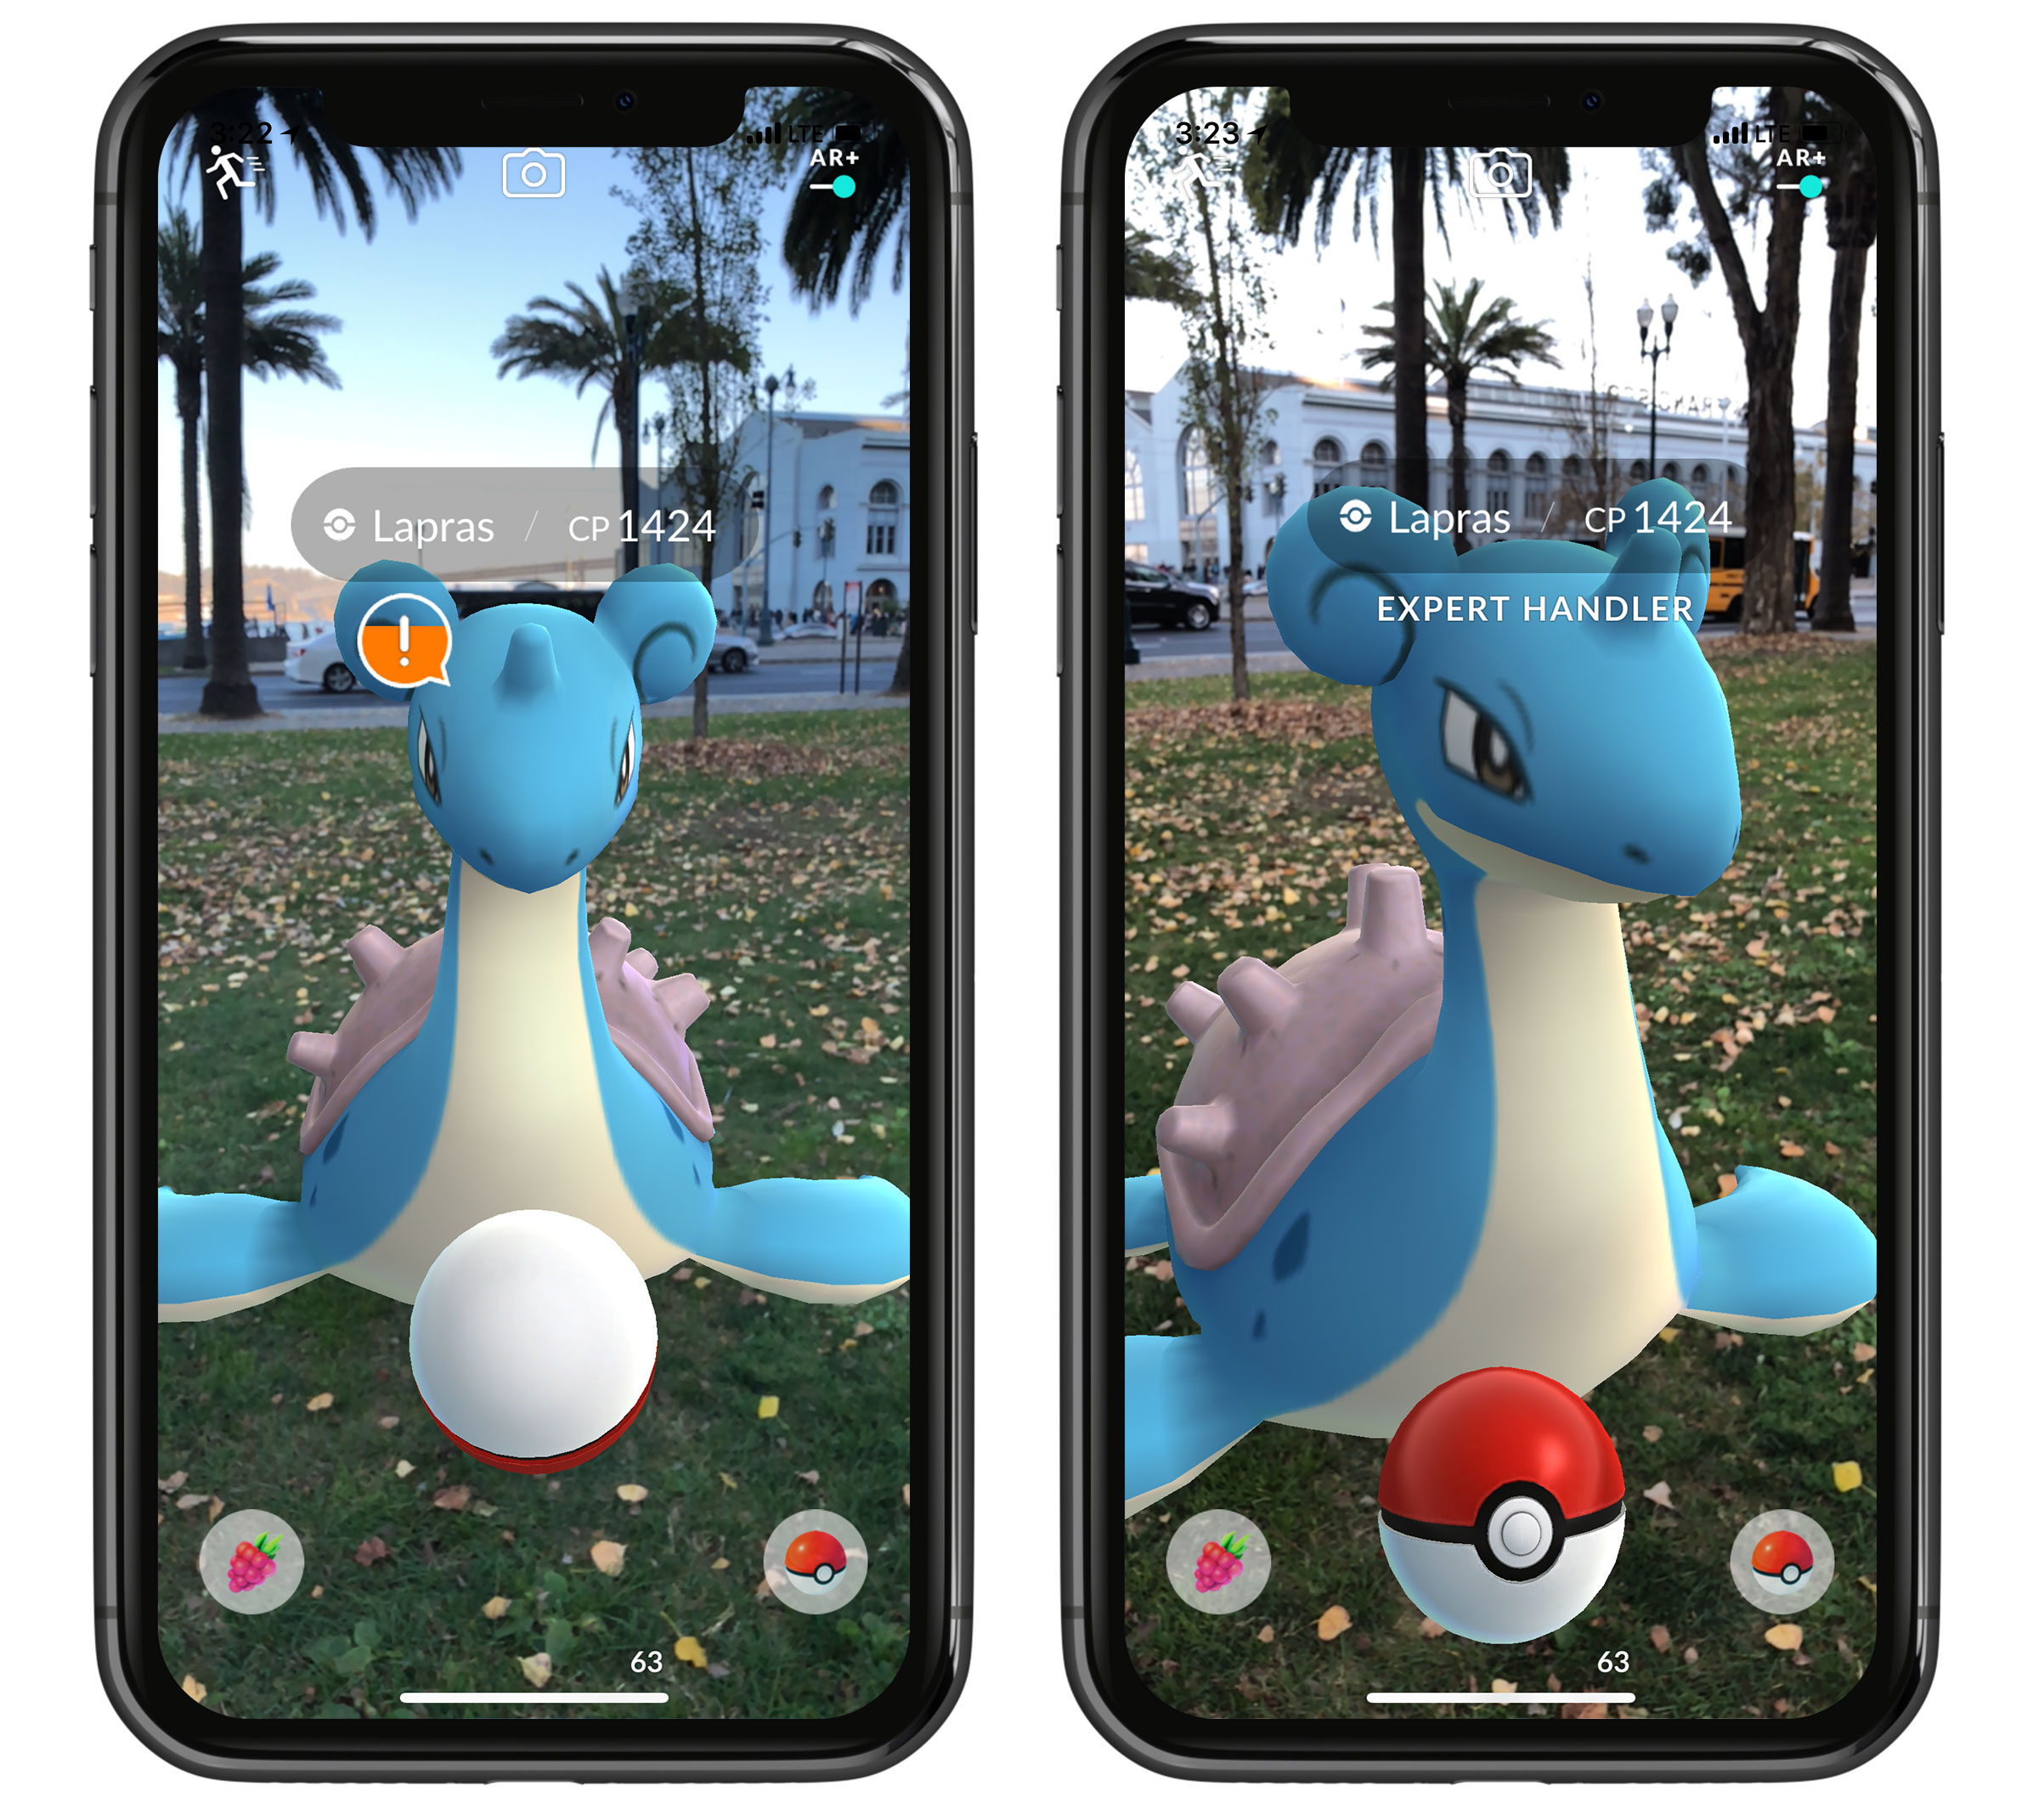
\includegraphics[width=0.45\textwidth]{images/pokemongo}
      \label{sub:STARGO}
      }
    \subfloat[Microsoft HoloLens - Vue au travers casque\protect\footnotemark]{
      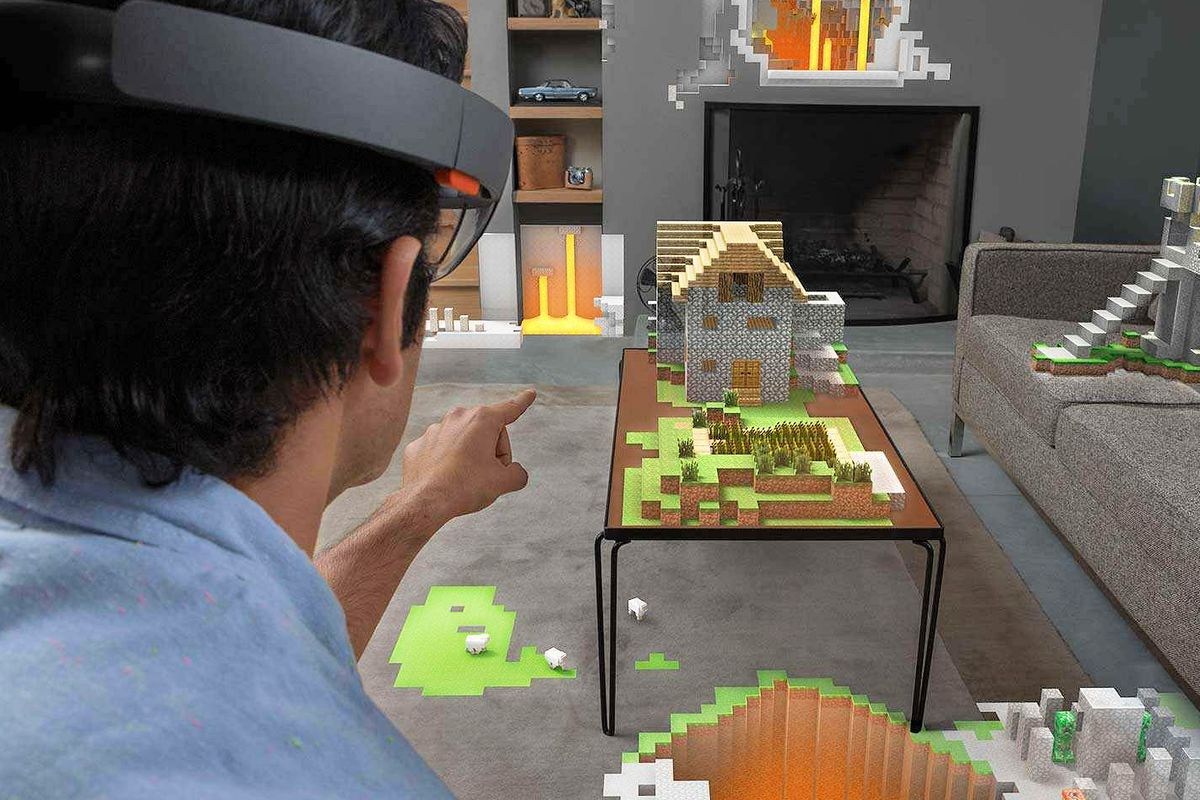
\includegraphics[width=0.45\textwidth]{images/hololens}
      \label{sub:STARHolo}
      }
\caption{Réalité augmentée vue au travers}
\label{fig:STAR}
\end{figure}
\footnotetext{Source: \href{https://pokemongolive.com/fr/}{Pokemon GO}}
\footnotetext{Source: \href{https://www.microsoft.com/fr-fr/hololens}{Microsoft HoloLens}}

\paragraph{Réalité augmentée spatiale}
% Trouver qui l'a inventé et quand
La réalité augmentée spatiale, plus communément appelé \emph{Spatial Augmented Reality (SAR)} est une technique de visualisation de la réalité augmentée se basant sur un dispositif de projection. Les éléments virtuels qui viennent "augmenter" le monde réel sont alors projetés dans l'espace (fig~\ref{fig:SAR}), d'où le terme spatiale. Cette notion d'augmentation de l'espace tend a rendre cette technologie naturellement collaborative car les projections ne dépendent pas d'un dispositif visuel et sont donc visibles par tout le monde. Ainsi la projectionEtant donné la méthode de visualisation est la visualisation directement sur les objets physiques manipulable ce qui permet de développer facilement des interfaces tangibles.

\begin{figure}[H]
\centering
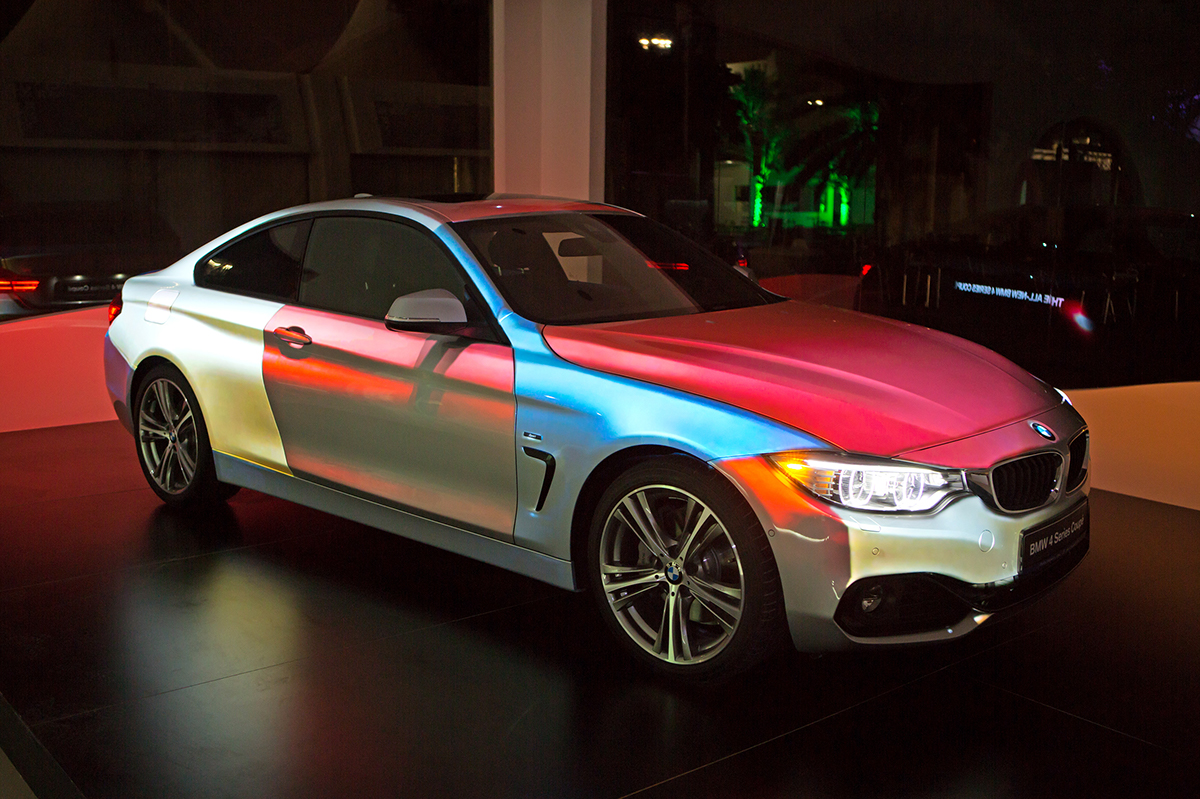
\includegraphics[width=0.5\textwidth]{images/SARMappingCar2}
\caption{Présentation d'une voiture en utilisant de la réalité augmentée spatiale\protect\footnotemark}
\label{fig:SAR}
\end{figure}
\footnotetext{Source: {Google Image}}

\paragraph{Interface tangible}
Une interface utilisateur tangible ou \emph{Tangible User Interface (TUI)} est une interface utilisateur via laquelle des objets physiques, ou encore le toucher, permettent de manipuler des données numériques (fig~\ref{sub:TUI}). Les interfaces utilisateurs tangibles remplacent très souvent les interfaces utilisateur graphiques (fig~\ref{sub:GUI}) où \emph{Graphical User Interface (GUI)} dans la plupart des application de réalité augmentée car elles fournissent un contrôle direct à l'utilisateur sur ce qu'il souhaite manipuler (par opposition au contrôle indirect, comme la souris, nécessaire à la manipulation des GUI).

\begin{figure}[H]
    \centering
	\subfloat[Interface Utilisateur Graphique (GUI)\protect\footnotemark]{
      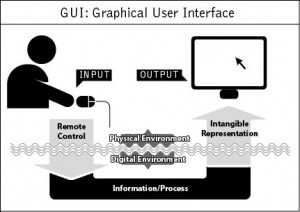
\includegraphics[width=0.45\textwidth]{images/GUI}
      \label{sub:GUI}
      }
    \subfloat[Interface Utilisateur Tangible (TUI)\protect\footnotemark]{
      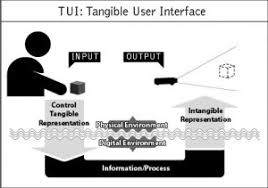
\includegraphics[width=0.45\textwidth]{images/TUI}
      \label{sub:TUI}
      }
\caption{Différences des interfaces utilisateurs}
\label{fig:GUITUI}
\end{figure}
\footnotetext{Source: \href{http://iconlibrary.iconshock.com/design/from-gui-to-tui/}{Icon Library - From GUI to TUI}}
\footnotetext{Source: \href{http://iconlibrary.iconshock.com/design/from-gui-to-tui/}{Icon Library - From GUI to TUI}}

\paragraph{Calcul haute performance}
Le calcul haute performance ou \emph{General-Purpose computing on Graphics Processing Units (GPGPU)} désigne une méthode de calcul utilisant la carte graphique (GPU) plutôt que le processeur (CPU). Cette technique permet de bénéficier de la puissance de la carte graphique afin de réaliser du calcul en parallèle et est très souvent utilisée pour la plupart des traitement lourd comme par exemple le rendu d'une scène 3D, l'encodage de vidéo, les simulations physiques (particules) etc. Cette technique repose sur le grand nombre de cœurs présent dans les cartes graphiques (contrairement aux processeurs) et sur la capacité de chacun de ces cœurs à effectué des opérations simples de manière très efficace. Le calcul haute performance ne peut cependant pas ce passer du CPU qui va être principalement utilisé pour récolter et transférer les données traités ou à traiter.
% Expliquer comment ca marche (carte graphique beaucoup de coeur pour faire des opérations simple, CPU pas beaucoup de coeur donc plus lent)
% Ajouter image comparaison

\begin{figure}[H]
\centering
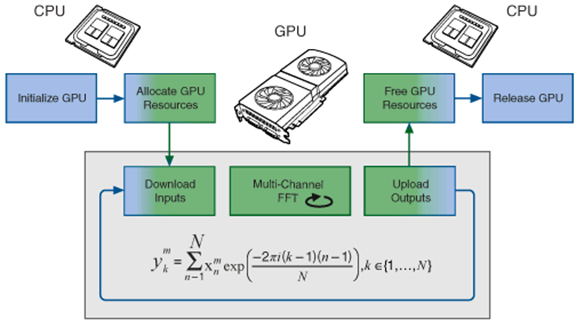
\includegraphics[scale=0.7]{images/gpuworkflow}
\caption{Exemple de calcul de la FFT sur GPU\protect\footnotemark}
\label{fig:gpgpu}
\end{figure}
\footnotetext{Source: \href{http://www.ni.com/white-paper/14077/fr/}{National Instruments}}
